\documentclass[12pt, a4paper]{report}
\usepackage[top=1cm, left=1cm, right=1cm]{geometry}

\usepackage[utf8]{inputenc}
\usepackage[russian]{babel}

\usepackage{array}
\newcolumntype{M}[1]{>{\centering\arraybackslash}m{#1}}

\usepackage{hyperref}
\hypersetup{
	colorlinks,
	citecolor=black,
	filecolor=black,
	linkcolor=black,
	urlcolor=black
}

\usepackage{sectsty}
\allsectionsfont{\centering}

\usepackage{indentfirst}
\setlength\parindent{24pt}

\usepackage{algorithm}
\usepackage[noend]{algpseudocode}

\usepackage{listings}
\usepackage{xcolor}
\definecolor{codegreen}{rgb}{0,0.6,0}
\definecolor{codegray}{rgb}{0.5,0.5,0.5}
\definecolor{codepurple}{rgb}{0.58,0,0.82}
\definecolor{backcolour}{rgb}{0.95,0.95,0.92}
\lstdefinestyle{mystyle}{
    backgroundcolor=\color{backcolour},   
    commentstyle=\color{codegreen},
    keywordstyle=\color{magenta},
    numberstyle=\normalsize\color{codegray},
    stringstyle=\color{codepurple},
    basicstyle=\ttfamily\footnotesize,
    breakatwhitespace=false,         
    breaklines=true,                 
    captionpos=b,                    
    keepspaces=true,                 
    numbers=left,                    
    numbersep=5pt,                  
    showspaces=false,                
    showstringspaces=false,
    showtabs=false,                  
    tabsize=2
}

\usepackage{graphicx}
\graphicspath{{plots/pictures/}}

\begin{document}
	\begin{titlepage}
		\begin{center}
			\large \textbf{Министерство науки и высшего образования Российской Федерации} \\
			\large \textbf{Федеральное государственное бюджетное образовательное учреждение высшего образования} \\
			\large \textbf{«Российский химико-технологический университет имени Д.И. Менделеева»} \\

			\vspace*{4cm}
			\LARGE \textbf{ОТЧЕТ ПО ЛАБОРАТОРНОЙ РАБОТЕ №1}

			\vspace*{4cm}
			\begin{flushright}
				\Large
				\begin{tabular}{>{\raggedleft\arraybackslash}p{9cm} p{10cm}}
					Выполнил студент группы КС-36: & Золотухин А.А. \\
					Ссылка на репозиторий: & https://github.com/ \\ 
					& MUCTR-IKT-CPP/ \\
					& ZolotukhinAA\_36\_ALG \\
					Принял: & Крашенников Роман Сергеевич \\
					Дата сдачи: & 17.02.2025 \\
				\end{tabular}

			\end{flushright}

			\vspace*{6cm}
			\Large \textbf{Москва \\ 2025}
		\end{center}
	\end{titlepage}
	
	\tableofcontents	
	\thispagestyle{empty}
	\newpage

	\pagenumbering{arabic}
	
	\section*{Описание задачи}
	\addcontentsline{toc}{section}{Описание задачи}
	\large
	В лабораторной работе предлагается изучить способ анализа алгоритма, связанный со временем. Рассмотреть для выбранного алгоритма сортировки наилучшее, наихудшее и среднее время и соотнести его с известным для алгоритма показателм эффективности O-большое. \par
	Допускается реализация задания на любом языке программирования, кроме лиспоподобных. Преподаватель может не знать конкретного языка реализации, поэтому вы должны быть способны объяснить алгоритм и нарисовать его без демонстрации непосредственно вашего кода. \par
	Задание:
	\begin{itemize}
		\item Реализовать метод сортировки: \textbf{Сортировка вставками};
		\item Реализовать проведения тестирования алгоритма сериями расчетов для измерения параметров За один расчёт выполняются следующие операции:
		\begin{itemize}
			\item Генерируется массив случайных значений;
			\item Запоминается время начала расчета алгоритма сортировки;
			\item Выполняется алгоритм сортировки
			\begin{itemize}
				\item Во время выполнения измерить количество повторных прохождений по массиву.
				\item Во время выполнения измерить количество выполнения операций обмена значений.
			\end{itemize}
			\item Вычисляется время, затраченное на сортировку: текущее время - время начала;
			\item Сохраняется время для одной попытки После этого расчёт повторяется до окончания серии.
			\begin{itemize}
				\item Алгоритм вычисляется 8 сериями по 20 раз за серию;
				\item Алгоритм в каждой серии вычисляется для массива размером M. (1000,2000, 4000, 8000, 16000, 32000, 64000, 128000);
				\item Массив заполняется значениями чисел с плавающей точкой в интервале от -1 до 1;
				\item Для серии запоминаются все времена, которые были замерены.
			\end{itemize}
		\end{itemize}
		\item По полученным данным времени построить графики зависимости времени от числа элементов в массиве:
		\begin{itemize}
			\item Совмещенный график наихудшего времени выполнения сортировки и сложности алгоритма, указанной в нотации O большое; \par
			Для построения графика вычисляется O большое для каждого размера массива. При этом при вычислении функции O(c * g(N)) подбирается такая константа c, чтобы при значении >1000 график O(N) был выше графика наихудшего случая, но второй график на его фоне не превращался в прямую линию.
			\item Совмещенный график среднего, наихудшего и наилучшего времени исполнения;
			\item График среднего количества обмена значений;
			\item График повторных обходов массива.
		\end{itemize}
		\item По результатам расчётов оформляется отчёт по предоставленной форме, в отчете:
		\begin{itemize}
			\item Приводится описание алгоритма;
			\item Приводится описание выполнения задачи (описание кода и специфических элементов реализации);
			\item Приводятся выводы (Графики и их анализ).
		\end{itemize}
	\end{itemize}

	\section*{Описание метода/модели}
	\addcontentsline{toc}{section}{Описание метода/модели}
	\large
	\textbf{Сортировка вставками} - это простой алгоритм сортировки, который работает путём итеративной вставки каждого элемента несортированного списка в его правильное положение в отсортированной части списка. Это похоже на сортировку игральных карт в ваших руках. Вы разделяете карты на две группы: отсортированные карты и несортированные карты. Затем вы выбираете карточку из несортированной группы и помещаете её в нужное место в отсортированной группе. \par
	Ход алгоритма:
	\begin{enumerate}
		\item Начинаем со второго элемента массива, поскольку предполагается, что первый элемент в массиве должен быть отсортирован;
		\item Сравниваем второй элемент с первым и проверяем, не меньше ли второй элемент, затем меняем их местами;
		\item Переходим к третьему элементу, сравниваем его с первыми двумя элементами и устанавливаем в правильное положение;
		\item Повторяем до тех пор, пока не будет отсортирован весь массив.
	\end{enumerate}
	Анализ сложности сортировки вставками:
	\begin{itemize}
		\item \textbf{Лучший вариант: O(\( N \))}, если список уже отсортирован;
		\item \textbf{Средний вариант: O(\( N^2 \))}, если список упорядочен случайным образом;
		\item \textbf{Наихудший вариант: O(\( N^2 \))}, если список находится в обратном порядке, \par
		где N - количество элементов в списке.
	\end{itemize}
	\begin{algorithm}
		\caption{Реализация алгоритма сортировки вставками}
		\begin{algorithmic}
			\State $i \gets 2$
			\While{$i \leq n - 1$}
				\State $j \gets i - 1$
				\While{$j \geq 0 AND A[j] > A[j + 1]$}
					\State $swap(A[j], A[j + 1])$
					\State $j \gets j - 1$
				\EndWhile
			\EndWhile
		\end{algorithmic}
	\end{algorithm}
	\textit{Преимущества}:
	\begin{itemize}
		\item Эффективно справляется с небольшими и почти отсортированными массивами;
		\item Экономит место;	
		\item Простой и легкореализуемый.
	\end{itemize}
	\textit{Недостатки}:
	\begin{itemize}
		\item Неэффективно справляется с большими массивами.
	\end{itemize}

	\section*{Выполнение задачи}
	\addcontentsline{toc}{section}{Выполнение задачи}
	Алгоритм сортировки вставками реализован на языке \textit{C++}. Построение графиков проводить с помощью программы \textit{GNUplot}.
	\lstset{style=mystyle}
	\begin{lstlisting}[language=C++]
		#include <iostream>
		int main() {
			std::cout << "Hello" << std::endl;
			return 0;
		}
	\end{lstlisting}
	\begin{figure}
		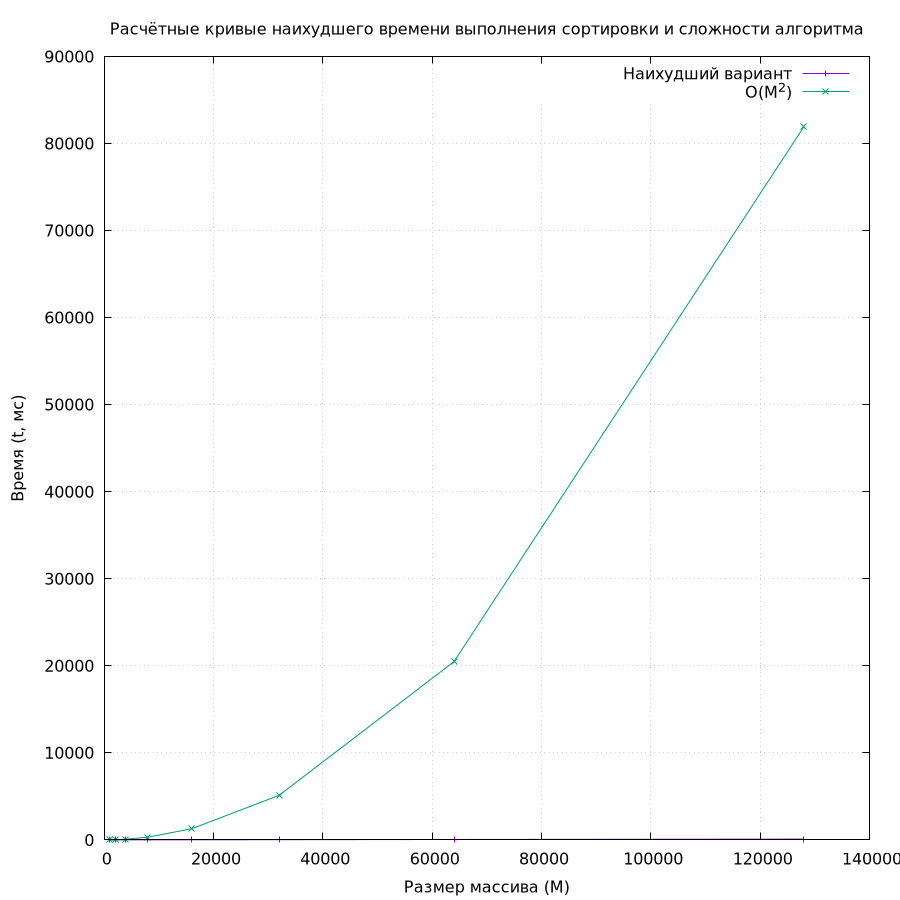
\includegraphics[width=500pt]{worst_and_complexity.png}
	\end{figure}
	\begin{figure}
		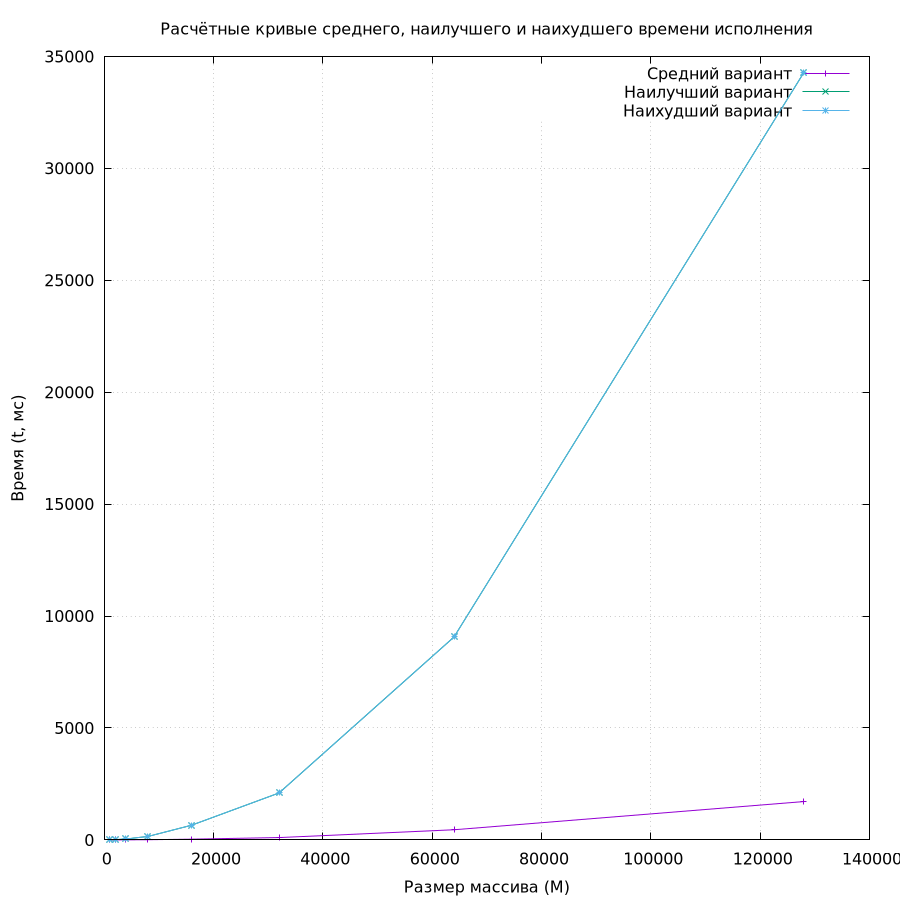
\includegraphics[width=500pt]{average_best_worst.png}
	\end{figure}
	\begin{figure}
		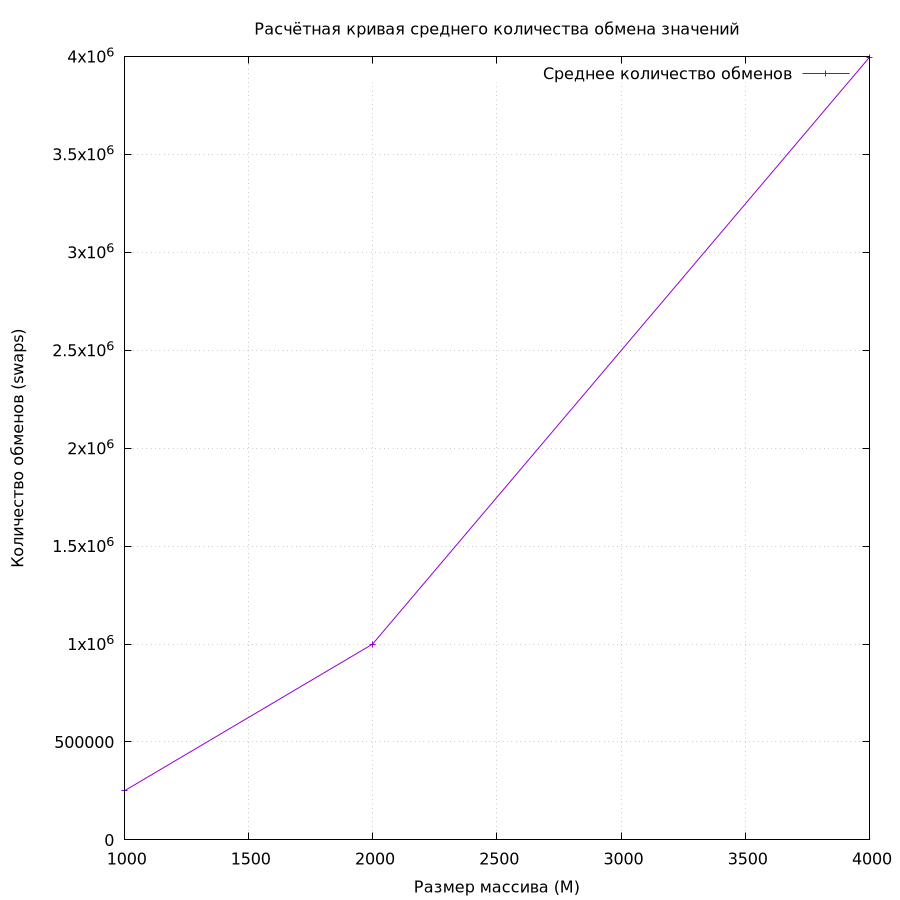
\includegraphics[width=500pt]{average_swaps.png}
	\end{figure}
	\begin{figure}
		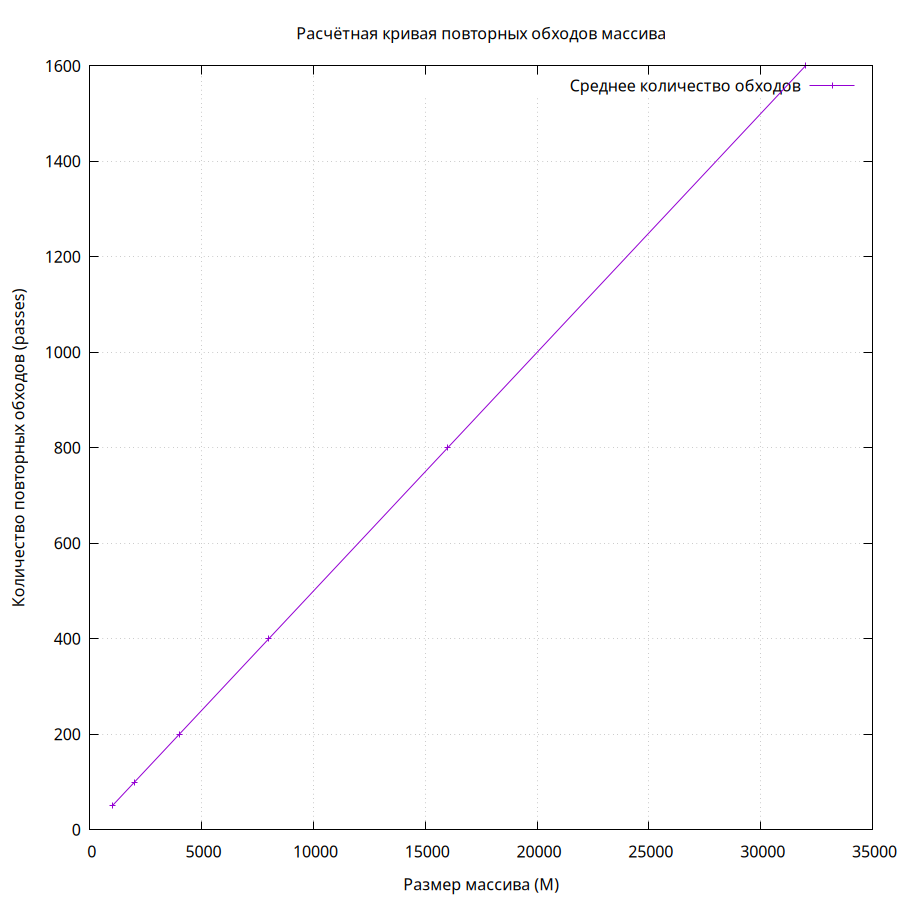
\includegraphics[width=500pt]{average_passes.png}
	\end{figure}

	\section*{Выводы}
	\addcontentsline{toc}{section}{Выводы}
		
\end{document}
